\documentclass[a4paper]{article}
\usepackage[utf8]{inputenc}
\usepackage{fullpage}
\usepackage{amsmath,amssymb}
\usepackage[colorlinks,linkcolor=blue]{hyperref} % use colored text in stead of ugly boxes
\usepackage[toc]{multitoc} % Nice two-column TOC

\usepackage{tabto}

\usepackage{pdfpages}
%~ TikZ is not in use in this document
%~ \usepackage{pgf}
%~ \usepackage{tikz}
%~ \usepackage{pictures/tikz-uml}

% new line after paragraph title.
\makeatletter
\renewcommand\paragraph{\@startsection{paragraph}{4}{\z@}%
  {-3.25ex\@plus -1ex \@minus -.2ex}%
  {1.5ex \@plus .2ex}%
  {\normalfont\normalsize\bfseries}}
\makeatother


\title{Programming Life - Final report}

\author{Group E:\\
Felix Akkermans \\
Niels Doekemeijer \\
Thomas van Helden \\
Albert ten Napel \\
Jan Pieter Waagmeester}

\begin{document}
\maketitle

\vfill

\small{\tableofcontents}
\pagebreak



\section{Introduction}


\section{Key problems and solutions - highlights}

During this project we have encountered some problems. In this section we will have a look at some of the highlights of these problems and how we fixed them.

Our program was developed test driven. This makes for very neat code, but it also comes with some problems. We mainly encountered problems with QUnit, a JQeury testing framework similar to Java's JUnit. Although the testing was done properly, the feedback on the results was not very helpful. Eventually we managed to tackle this problem with some extra manual testing.

A common issue using server-client structure is the actual connection between the two. In the beginning we had some trouble with this but this was mainly caused by out of sync code and trouble with Apache Tomcat. We decided on a standard version of Tomcat and wrote a setup page on the wiki. Afterwards, the problem was solved.

Another problem client side was the dragging and dropping of gates and connecting them with wires. We had anticipated this as being tough and found a solution in jsPlumb, a solution with its downsides. The framework jsPlumb makes it easy to create connectors and draw wires between gates, but it didn't fully meet our needs so we had to customize it, leading to quite some hours of extra work. (NIELS MORE EXPLANATION)

At one point, we figured we wanted to select our proteins from dropdown menus on our wires. Regular dropdown menus from Javascript are not an issues, however combining this with jsPlumb and bootstrap proved to be a little more difficult. This took more time than we had anticipated but was eventually solved after trying several options.

Throughout this project we worked with Git and GitHub to share our code. We also used the ticket mechanism of GitHub to keep track of what had to be done. Git is exceptionally good at merging code but cannot always prevent conflicts. If there is too little communication between two people who are working on the same code, merging can become difficult. However, with some reverts and recommitting these problems were resolved.

Towards the end of our project, we did some major restructuring. We shifted some functions around, changed some names and did some more testing and commenting. We did this based on the feedback we got from the SIG evaluation. The biggest changes were made on the client side.

Our program is not only to model circuits but also to calculate and display the outcome. We displayed the outcome in a graph, but this showed some weird results. It turned out that the solver for our circuits had some issues (ALBERT EXPLAIN HOW IT WAS SOLVED).


\section{Reflection on the teamwork}

\section{Individual reflection on the project} %max 1 A4 per teammember
\subsection{Felix Akkermans}
\subsection{Niels Doekemeijer}
\subsection{Thomas van Helden}
\subsection{Albert ten Napel}
\subsection{Jan Pieter Waagmeester}

\section{Lightweight SCRUM Plans}
The following pages will include the relevent parts of our lightweight scrumplans for each iteration. The colored links and numbers with a hashtag refer to GitHub issues on \url{https://github.com/FelixAkk/synthbio/issues}. For each iteration, a milestone is available providing a nice overview of the issues for each iteration.

\includepdf[
	landscape, frame, nup=1x2, pages=2-3,
	addtotoc={2 , subsection , 1 , Scrumplan 1 , scrum-1}
]{../scrumplan-1/scrumplan-1.pdf}

\includepdf[
	landscape, frame, nup=1x2, pages=2-3,
	addtotoc={2 , subsection , 1 , Scrumplan 2 , scrum-2}
]{../scrumplan-2/scrumplan-2.pdf}

\includepdf[
	landscape, frame, nup=1x2, pages=2-3,
	addtotoc={2 , subsection , 1 , Scrumplan 3 , scrum-3}
]{../scrumplan-3/scrumplan-3.pdf}


\end{document}
